% !TeX spellcheck = en_US
\chapter{Probabilities}
\label{cha:probabilities}
For more examples, exercises with solutions, check:
\begin{itemize}
	\item \citeaustitle{bishop2006pattern}
\end{itemize}

\section{General}
\subsection{Basic Definitions}
\begin{itemize}
	\item If $x$ is discrete: $\underset{x}{\sum} p(x) = 1$ with $\forall$ $0 \leq p(x) \leq 1$
	\item If $x$ is continuous: $\displaystyle \int p(x) \,dx = 1 \Rightarrow \exists$ a \textbf{\ac{pdf}}\\
	$p(x)$ can take any positive value, as long as \(\displaystyle \int p(x) \,dx = 1\) \tab 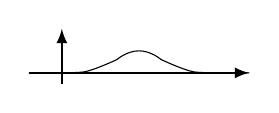
\begin{tikzpicture}[scale=1.4]
		\draw[-latex, thick] (-1,0)--(1,0);
		\draw[-latex, thick] (-.7,-.1)--(-.7,.4);		
		\draw plot [smooth, tension=1] coordinates {(-.2,.121) (0,.2) (.2,.121)};
		\draw plot [smooth, tension=.4] coordinates {(-1,0) (-.5,.00876) (-.2,.121)};
		\draw plot [smooth, tension=.4] coordinates {(.2,.121) (.5,.00876) (1,0)};
	\end{tikzpicture}	
	\note: theoretically $p(x) = 0, \forall x$
	\item Common types
	\begin{align*}
		& \text{Joint probability:} 		&& p(x_i, y_i) 	&& = p(X=x_i, Y=y_i) \\
		& \text{Marginal probability:} 		&& p(x_i) 		&& = p(X=x_i) \\
		& \text{Conditional probability:} 	&& p(y_i | x_i) && = p(Y=y_i|X=x_i)
	\end{align*}	
	\item Sum rule: $\displaystyle \sum$ joint \ac{prob} = marginal \ac{prob}\\
	$\Rightarrow$ Marginalization	
	\begin{itemize}
		\item discrete variable: $\displaystyle p(x)=\underset{y}{\sum} p(x, y)$
		\item continuous variable: $\displaystyle p(x) = \int p(x,y) dy$
	\end{itemize}
	\item Product rule: Product of marginal \ac{prob} and conditional \ac{prob} = joint \ac{prob}
\end{itemize}

\subsection{Expectation}
\label{subsec:expectation}
\begin{align*}
	& \text{For variable $x$:} && \expectation{x} = \underset{x}{\sum}x.p(x) && = \int p(x)x\text\ {d}x \\
	& \text{For function $f(\cdot)$:} && \expectation{f(x)} = \underset{x}{\sum}f(x).p(x) && = \int p(x)f(x)\ \text{d}x
\end{align*}

\subsection{Independence and Variability}
\begin{itemize}
	\item Independence. \Eg: $x, y$ are independent, then
	\[\begin{cases}
		p(x|y) = p(x)\\
		p(y|x) = p(y)
	\end{cases}
	\Leftrightarrow p(x,y) = p(x).p(y)\]	
	\item Variability
	\begin{itemize}
		\item variance: how much variability there is in $f(x)$ around its mean value $\expectation{f(x)}$\\
		$var [f] = \expectation{\left(f(x)-\expectation{f(x)}\right)^2} = \expectation{f(x)^2} - \expectation{f(x)}^2$
		\item covariance: for two random variables $x, y$\\
		$cov [x, y] = \mathbb{E}_{x,y}\left[xy\right] - \expectation{x}.\expectation{y}$
		\item covariance matrix: if $x, y$ are vectors
		\begin{align*}
			cov [\textbf{x}, \textbf{y}] &= \mathbb{E}_{\textbf{x},\textbf{y}} \left[ \left\{\textbf{x}-\expectation{\textbf{x}}\right\} \left\{\textbf{y}^T -  \expectation{\textbf{y}^T} \right\} \right]\\
			&= \mathbb{E}_{\textbf{x,y}}\left[\textbf{xy}^T\right] - \expectation{\textbf{x}}.\expectation{\textbf{y}^T}
		\end{align*}
	\end{itemize}
\end{itemize}

\subsection{Bayes Rule}
\label{subsec:bayes-rule}
\begin{align*}
	& p(x_i|y_i).p(y_i) = p(y_i|x_i).p(x_i) = p(x_i, y_i) \\
	\Rightarrow\; &p(y_i|x_i) = \frac{p(x_i|y_i).p(y_i)}{p(x_i)} = \frac{p(x_i|y_i).p(y_i)}{\underset{y}{\sum} p(x_i|y_i).p(y_i)}
\end{align*}
$\Rightarrow$ the \hlb{Bayes equation}:\tab{\color{red} \boxed{\hlre{posterior = \frac{likelihood \times prior}{normalization~factor}}}}

\section{Types of Probability Distributions}
Reference source: \href{https://machinelearningcoban.com/2017/07/09/prob/}{machinelearningcoban.com}.
\subsection{Bernoulli Distribution}
Bernoulli Distribution is a distribution to describe binary discrete variables. It's the case that the variable can only take value in 2 classes $x \in \{0,1\}$. \Eg, the probability of throwing a coin. The Bernoulli distribution is defined with parameter $\lambda \in[0,1]$:
\begin{equation}
	p(x) = \text{Bern}_x[\lambda] = \begin{cases}
		p(x=1) = \lambda\\
		p(x=0) = 1-\lambda
	\end{cases}
\end{equation}
In short form, the above equation can be combined into one:
\begin{equation}
	p(x) = \lambda^x(1-\lambda)^{(1-x)} \Rightarrow
	\begin{cases}
		p(0) = \lambda^0 (1-\lambda)^1 = 1-\lambda \\
		p(1) = \lambda^1 (1-\lambda)^0 = \lambda \\
	\end{cases}
\end{equation}

\subsection{Categorical Distribution}
\label{subsec:categorical-distribution}
\textit{Categorical Distribution} is the generalization of \textit{Bernoulli Distribution} for $K$ classes of the discrete variable $x \in \{ 1, 2, \dots, K\}$. Accordingly, there will be $K$ parameters to describe this \ac{pdf}: $\lambda = [\lambda_1, \lambda_2, \dots, \lambda_K]$, with $\lambda_k \geq 0$ and $\sum \lambda_k = 1$. Each $\lambda_k$ represents the probability to take the output $k$: $p(x = k) = \lambda_k$. In short: $p(x) = \text{Cat}_x [\lambda]$.

Another common way to represent the output is the one-hot vector, $\mathbf{x} \in \{\mathbf{e}_1, \mathbf{e}_2, \dots, \mathbf{e}_K\}$ with $\mathbf{e}_k$ is the $k$-unit vector, which has all 0-element, except the $k$-element equal to 1. \Eg, given 3 classes: $\textbf{e}_1 = [1, 0, 0]^T, \textbf{e}_2 = [0, 1, 0]^T, \textbf{e}_3 = [0, 0, 1]^T$. We will then have:
\begin{equation}
	p(\mathbf{x} = \mathbf{e}_k) = \prod_{j=1}^K \lambda_j^{x_j} = \lambda_k
\end{equation}
because for $\textbf{x}=\textbf{e}_k$, only $x_k=1$, while $x_j = 0, \forall j\neq k$.

\subsection{Univariate Normal Distribution}
Univariate Normal Distribution is also known as the Gaussian distribution. For single dimension data (in 1D): $x \in (-\infty, \infty)$, the mean $\mu \in \mathbb{R}$, and the variance $\sigma^2$ with $\sigma \in \mathbb{R}$.
\begin{equation}
	p(x) = \text{Norm}_x\left[\mu, \sigma^2\right] = \mathcal{N}(\mu, \sigma^2) = \frac{1}{\sqrt{2\pi\sigma^2}}.\text{exp}\left(-\frac{(x-\mu)^2}{2\sigma^2}\right)
\end{equation}
\note
\begin{itemize}
	\item \hlr{Marginals \ac{prob} of Gaussian are again Gaussian.}
	\item When estimating the \ac{param} of a Gaussian, beware the underestimation problem.
	\begin{align*}
		\expectation{\mu_{ML}} &= \mu \\
		\expectation{\sigma^2_{ML}} &= \left(\frac{N-1}{N}\right)\sigma^2 \\
		\Rightarrow \overset{\sim}{\sigma}^2 &= \left(\frac{N}{N-1}\right)\sigma^2_{ML} = \frac{1}{N-1} \sum_{n=1}^{N} (x_n-\hat{\mu})^2
	\end{align*}
\end{itemize}
\begin{figure}[hbt!]
	\centering
	\includegraphics[width=0.7\textwidth]{gaussian-pdf.png}
	\caption{Bivariate Gaussian distribution (\href{https://stats.stackexchange.com/questions/102632/plot-two-dimensional-gaussian-density-function-in-matlab}{src}).}
	\label{fig:relation-ai-ml-dl}
\end{figure}

\subsection{Multivariate Normal Distribution}
\textit{Multivariate Normal Distribution} is the extension of \textit{Univariate Normal Distribution} to multi-dimensional data: $\textbf{x}, \boldsymbol{\mu} \in \mathbb{R}^D, \sigma^2 \Rightarrow \Sigma \in \mathbb{S}^D_{++}$ ($\mathbb{S}^D_{++}$ is the set of positive definite symmetric matrix)
\begin{equation}
	p(x) = \text{Norm}_x [\boldsymbol{\mu}, \Sigma] = \mathcal{N}(\boldsymbol{\mu}, \Sigma) = \frac{1}{2\pi^{D/2}| \Sigma|^{\frac{1}{2}}} . \text{exp} \left( -\frac{1}{2} {(\textbf{x} - \boldsymbol{\mu})^T \Sigma^{-1} (\textbf{x} - \boldsymbol{\mu})} \right)
\end{equation}

\subsection{Beta Distribution}
This distribution describes the parameter for another distributions. \Eg, Dirichlet \ac{pdf} describes Categorical Distribution (\subsecref{subsec:categorical-distribution})